\section{Borderless: Twitter Misinformation and Political Communities}
In this section, we analyze the interplay between the penchant towards political polarization, toxicity, and misinformation on social media users. Previous works have indicated that toxicity levels are heavily tied with users' political polarization levels~\cite{chipidza2021effect,kim2021distorting} as well as their penchant to conspiratorial content~\cite{hanley2021no}. We now investigate how toxic and political polarized communities contribute to the propagation of misinformation and conspiracies by individuals users on Twitter.  

\begin{figure}
\centering
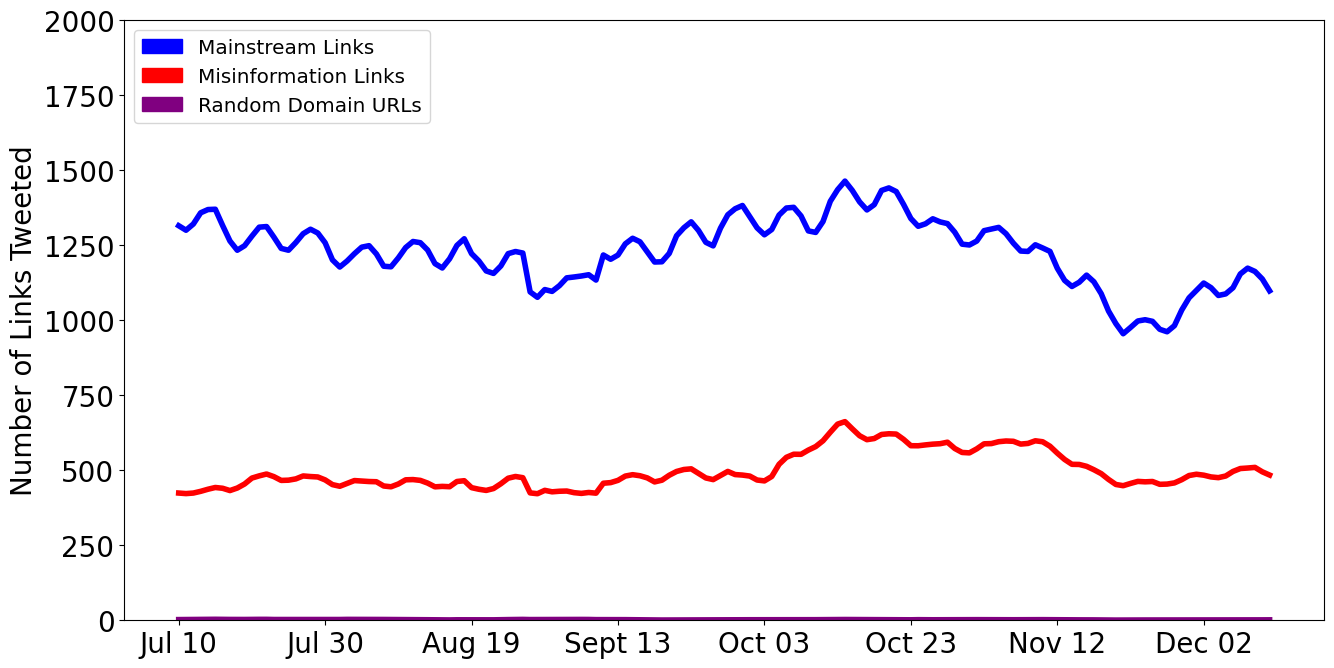
\includegraphics[width=\columnwidth]{figures/LevelsOfMisinformationAndNewsOnTwitter.png} 
\caption{\textbf{Number of Authentic News, Misinformation, and Conspiracy Theory Links on Twitter in 2020}--- Misinformation maintains a large presence of Twitter, with about half as many links as authentic news. Conspiracy websites having a relatively small but non-negligible presence on the platform. 
}
\label{figure:levels_of_misinfo}
\end{figure}

As seen in Figure~\ref{figure:levels_of_misinfo}, counting the number of instances of misinformation, authentic news, and conspiracy theory hyperlinks based on a 1\% Twitter sampling over 6 months, there are consistent levels of misinformation news articles tweeted. The amount of misinformation links from users, in fact largely follows the amount of authentic news tweeted. Specifically, we find a Pearson correlation of 0.711 between the number of misinformation URLs posted and the number of authentic news posted.  At any given time, the amount of misinformation links within our dataset varies from, $\frac{1}{3}$ to $\frac{1}{2}$ of the amount of authentic news hyperlinks posted. Comparing this to a set of non-news related URLS as well as a set of random domains (chosen randomly from the Amazon Alexa Top 1M from January 1 2022), we see that the changing amounts of misinformation and news based URLs in our dataset is largely due to the vicissitudes of the news cycles rather than as an artifact of our dataset. 

Having established the relative levels of misinformation on Twitter, we now seek to understand some of the drivers behind misinformation heavy Twitter accounts. Taking all URLS within our dataset, we acquire 189K different Twitter accounts that tweets authentic news, misinformation, or conspiracy theories during the month of January. Within this set of Twitter accounts 139663 accounts tweeted at least one authentic news website and 115073 accounts tweeted at least one misinformation website. Using the Tweepy API, we collect the last 3240 tweets of each of these users, giving us a dataset of 446,439,819 tweets total. 

\begin{figure*}
\begin{subfigure}{.25\textwidth}
  \centering
  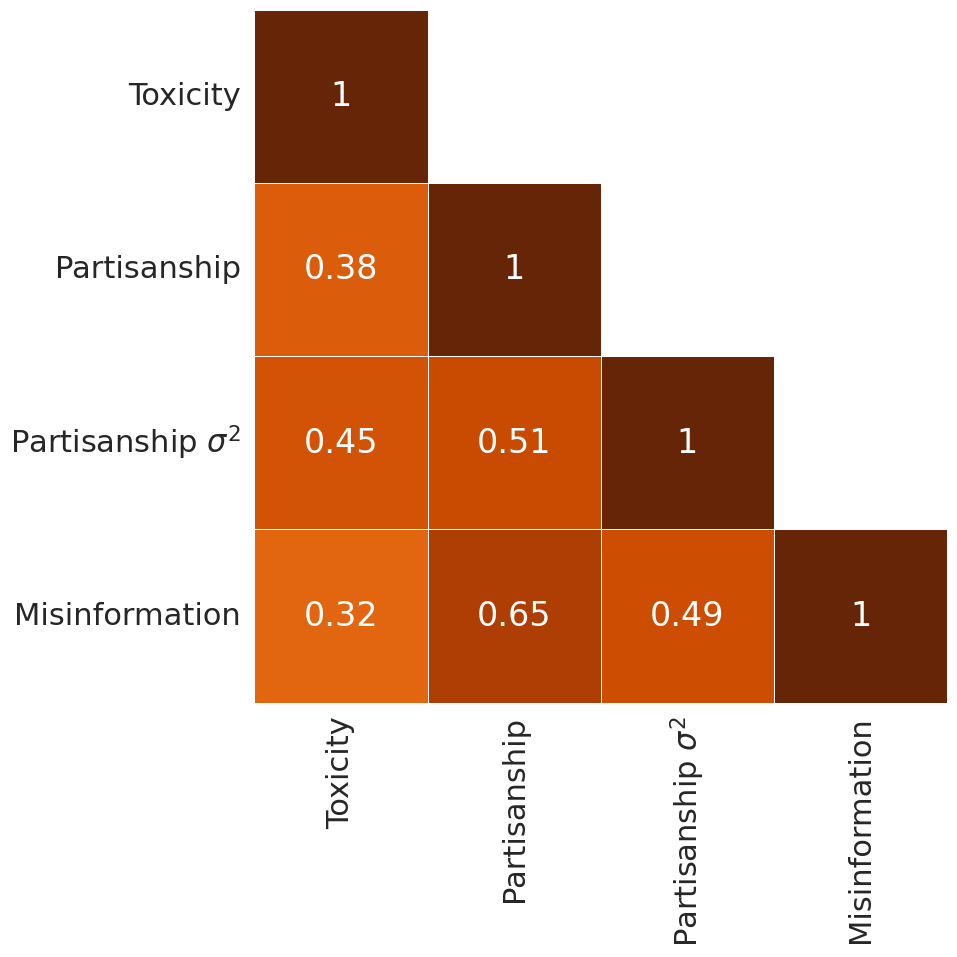
\includegraphics[width=1\linewidth]{figures/all-correlations.png}
  \caption{All User Correlations}
\label{fig:twitter-reddit-partisanship-time}
\end{subfigure}%
\hspace{20pt}
\begin{subfigure}{.25\textwidth}
  \centering
  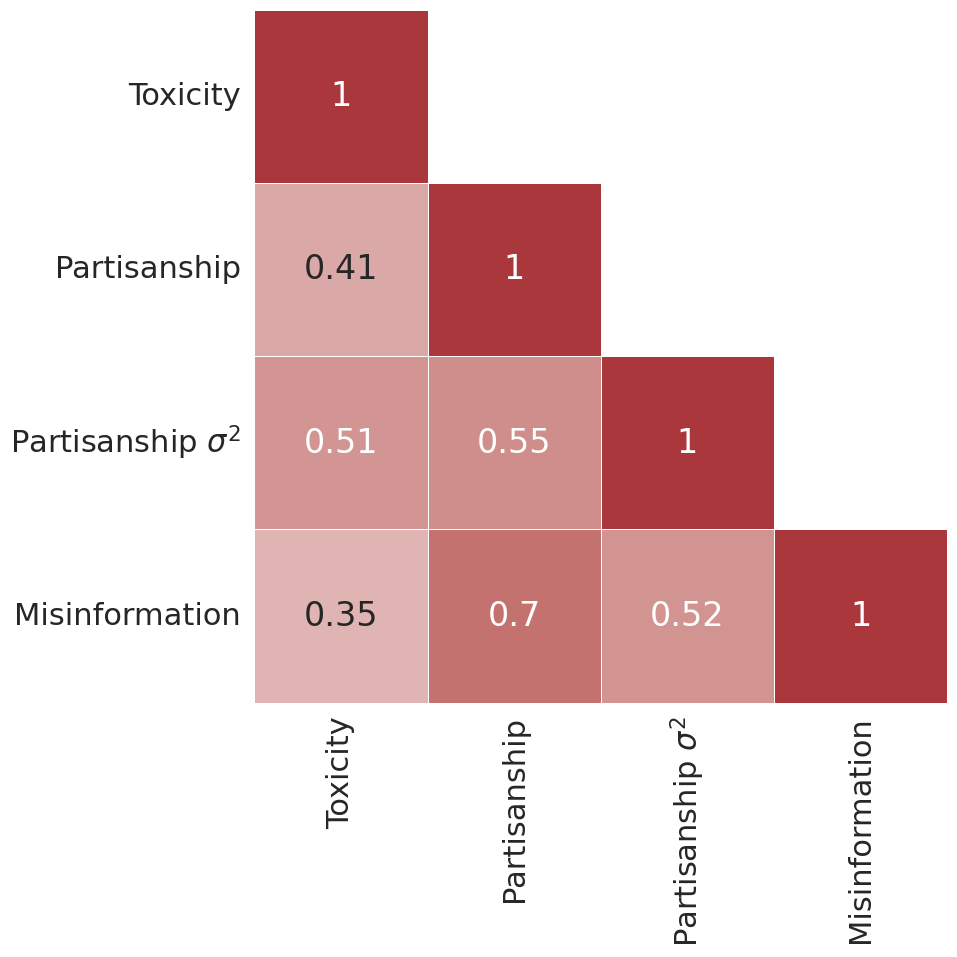
\includegraphics[width=1\linewidth]{figures/republican-correlations.png}
  \caption{Republican User Correlations}
  \label{fig:twitter-reddit-partisanship}
\end{subfigure}
\hspace{20pt}
\begin{subfigure}{.25\textwidth}
  \centering
  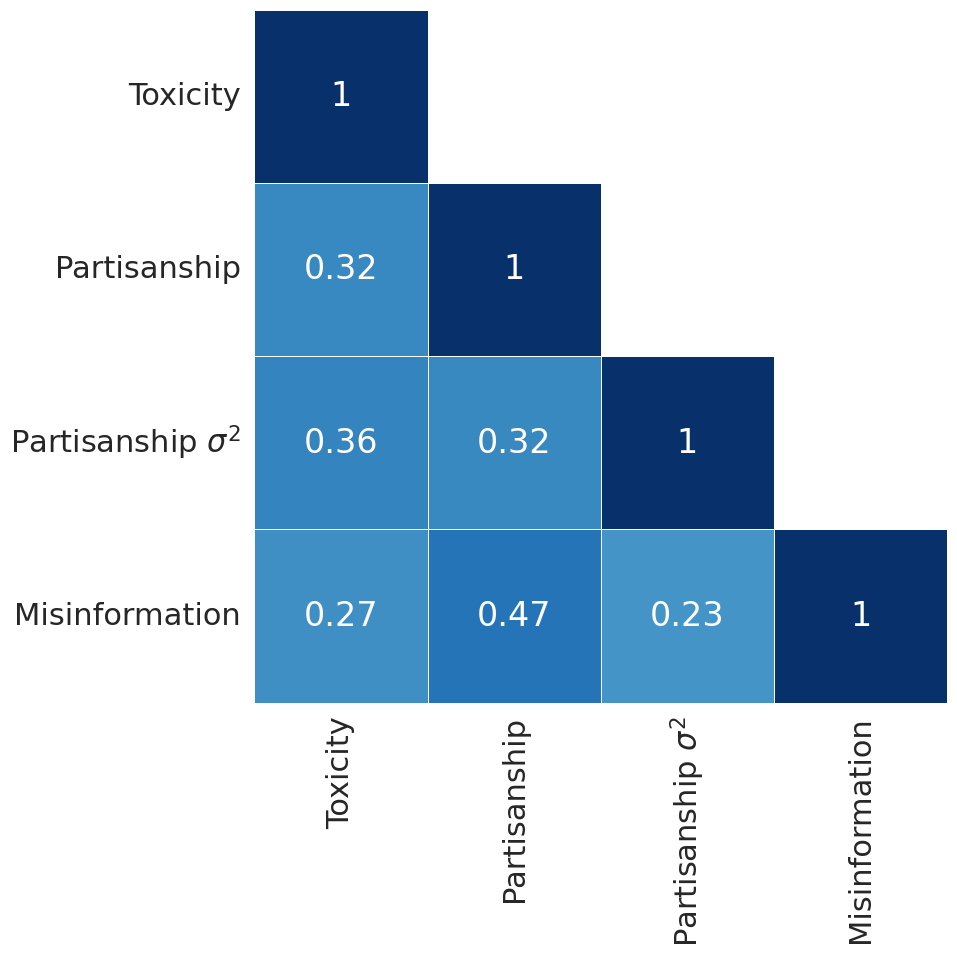
\includegraphics[width=1\linewidth]{figures/democratic-correlations.png}
  \caption{Democratic User Correlations}
  \label{fig:twitter-reddit-toxicity-time}
\end{subfigure}
\caption{\textbf{Twitter User Characteristic Correlations}--- Among different 
}
\label{fig:twitter-correlations}
\end{figure*}

After labeling each tweet with the Perspective API and gathering each accounts approximate partisanship, partisanship URL variance, and misinformation promotion levels, we now seek to understand the factors behind accounts promoting misinformation. As a proxy for the misinformation promotion level of given Twitter users, we utilize the percentage of the URLs that they post that belong to our set of misinformation domains.

As seen in Figure~\ref{fig:twitter-correlations}, there is a high degree of correlation between the political polarization of users and misinformation levels of users. This largely concurs with prior research that suggests that political polarization is the most potent reason behind the sharing of ``fake-news'' on Twitter~\cite{osmundsen2021partisan}. Looking at users whose average URL posted is conservative/Republican, this is especially prominent,  with polarization having a 0.70 Pearson correlation with levels of misinformation on their accounts. 


We also see, somewhat counter-intuitively, at a given level of partisanship, as the partisanship variance of individuals accounts increases, the amount of misinformation that that account post also increases. This suggests that users that actually engage with materials/hyperlink to materials that are substantially different from the average political information that they hyperlink to are more likely to post misinformation. Bucking our initial expectations, engaging with more and different sources is associated with heavier amounts of misinformation. Prior work~\cite{starbird2018ecosystem} has noted the political echo chambers that promote misinformation online. However, this appears to be only a part of the story of the spread of misinformation. 
\begin{comment}
\begin{figure}
\centering
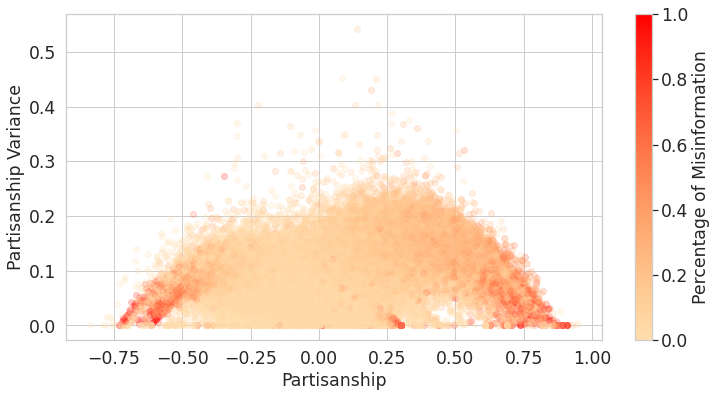
\includegraphics[width=\columnwidth]{figures/misinformation-graph-partisan-var.png} 
\caption{\textbf{Partisanship and Partisanship Variance Affect on Misinformation}--- As users become more politically hardened and engage with a higher amount of news sources, they are more likely to post misinformation. While not exact, as levels of variety of political URLS posted increases at each level of partisanship, the the levels of misinformation increases as well. This is seen by the red fraying at the edges of the graph.  
}
\label{figure:partisanship-misinfo-variance}
\end{figure}
\end{comment}
As seen in Figure~\ref{figure:partisanship-misinfo-variance}, it is the set of users that have the highest variance of political URLs as well as the most highly partisan users that have the highest levels of misinformation on their Twitter accounts.For example one particularly highly misinformation-dense account (Figure~\ref{fig:twitter-misinformation2}) linked to a video from MSNBC to deride one of its hosts. This is not to say that these users regularly link to highly opposing views often; however, this tendency to interact with substantially different than a user's political average results in a higher likelihood of misinformation. 
\begin{figure*}
\begin{subfigure}{.48\textwidth}
  \centering
  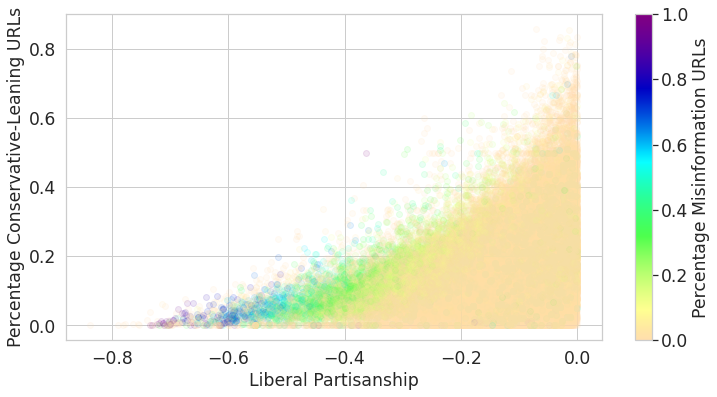
\includegraphics[width=1\linewidth]{figures/liberal-graph-partisan-misinformation.png}
\label{fig:left-twitter-pol-toxicity}
\end{subfigure}%
\begin{subfigure}{.48\textwidth}
  \centering
  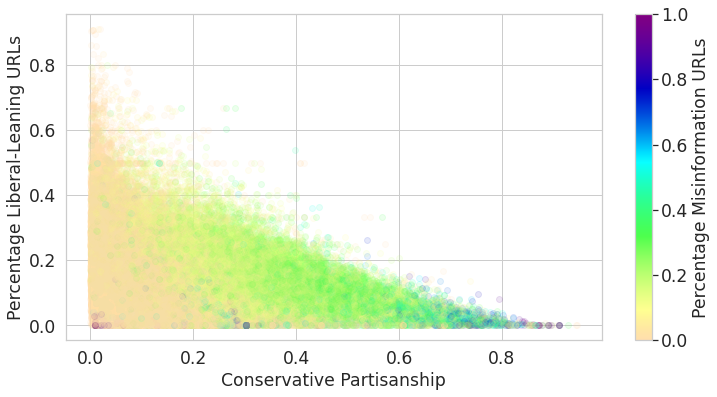
\includegraphics[width=1\linewidth]{figures/conservative-graph-partisan-misinformation.png}
  \label{fig:right-twitter-pol-toxicity}
\end{subfigure}
\caption{\textbf{Average Misinformation Levels as a function of average political bias and tendency to post opposing views}-- Users that post the URLs of websites that are against their average political bias are more likely to post misinformation.
}
\label{fig:twitter-pol-toxicity}
\end{figure*}

Users that post more URLs that are opposed to their mean political URLs/belief also show a higher probability of toxicity compared to other users of similar political averages. Plotting levels of toxicity as a function of political bias and the tendency to post opposing views (URLs from websites that are conservative-leaning for Democratic voters and vice versa), we see 1) that levels of toxicity are highly connected with levels of partisanship ( Pearson correlation of 0.38 for all users), and 2) that as the number of URLs from websites with opposing views increases, we see that average levels of toxicity increase as well. Looking at Figure \ref{fig:twitter-pol-toxicity} and , we  that for both left-wing and right-wing users, similarity at each given partisanship level, as the percentage of URLs from websites that oppose their mean political bias increases, that mean levels of toxicity increases with users at the end of each level of partisanship showing the highest levels of toxicity. For liberal leaning users, we find that after normalizing for partisanship, a Pearson correlation of 0.242 between the average toxicity of a user and their tendency to post URLs opposing their political bias. Just looking at decidedly conservative users with an average political bias of 0.1 or greater, this correlation increases to 0.302. For conservative users, we find that after normalizing for partisanship, the tendency to post opposing views accounts, has a Pearson correlation of 0.240 with their average toxicity. Just looking at decidedly conservative users with an average political bias of 0.1 or greater, this correlation increases to 0.302. As seen, users with the tendency to post URLS against their political bias have higher associated levels of toxicity. This largely mirrors  the tendency to also post misinformation as previously discussed. 

\begin{figure*}
\begin{subfigure}{.3\textwidth}
  \centering
  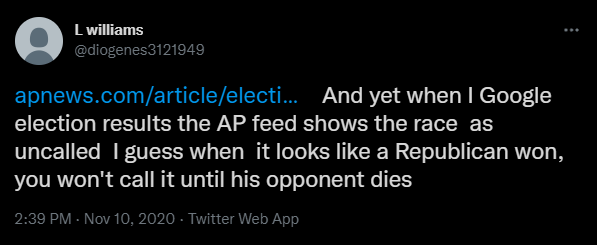
\includegraphics[width=1\linewidth]{figures/high-var-user-tweet1.png}
\label{fig:twitter-misinformation1}
\end{subfigure}%
\begin{subfigure}{.3\textwidth}
  \centering
  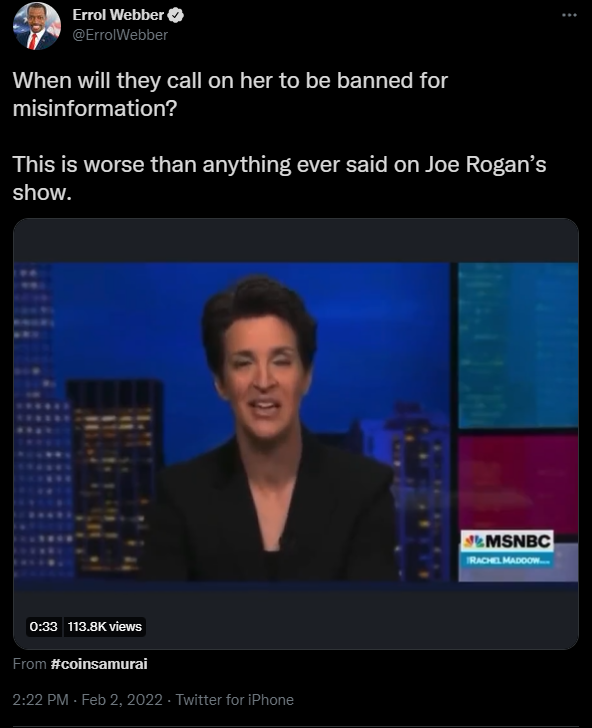
\includegraphics[width=1\linewidth]{figures/high-var-user-tweet2.png}
  \label{fig:twitter-misinformation2}
\end{subfigure}
\begin{subfigure}{.3\textwidth}
  \centering
  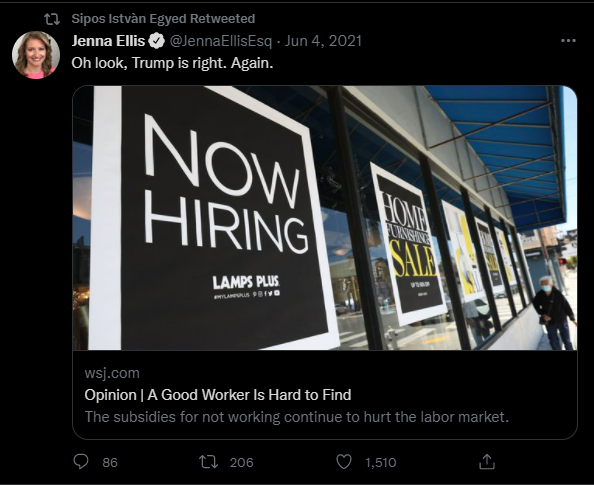
\includegraphics[width=1\linewidth]{figures/high-var-user-tweet3.png}
  \label{fig:twitter-misinformation3}
\end{subfigure}
\caption{\textbf{Examples of partisan users engaging with material from across the political aisle }-- Highly partisan and misinformation dense Twitter accounts occasional respond to and engage with news stories from authentic news. As pictured, users often deride these sources or cite that stories are  highly divisive.
}
\label{fig:twitter-misinformation-levels}
\end{figure*}

%% Likelihood to post a right-leaning URL if left wing vs probability to post a left-wing URL if right leaning as a function of partisanship 
\begin{figure*}
\begin{subfigure}{.24\textwidth}
  \centering
  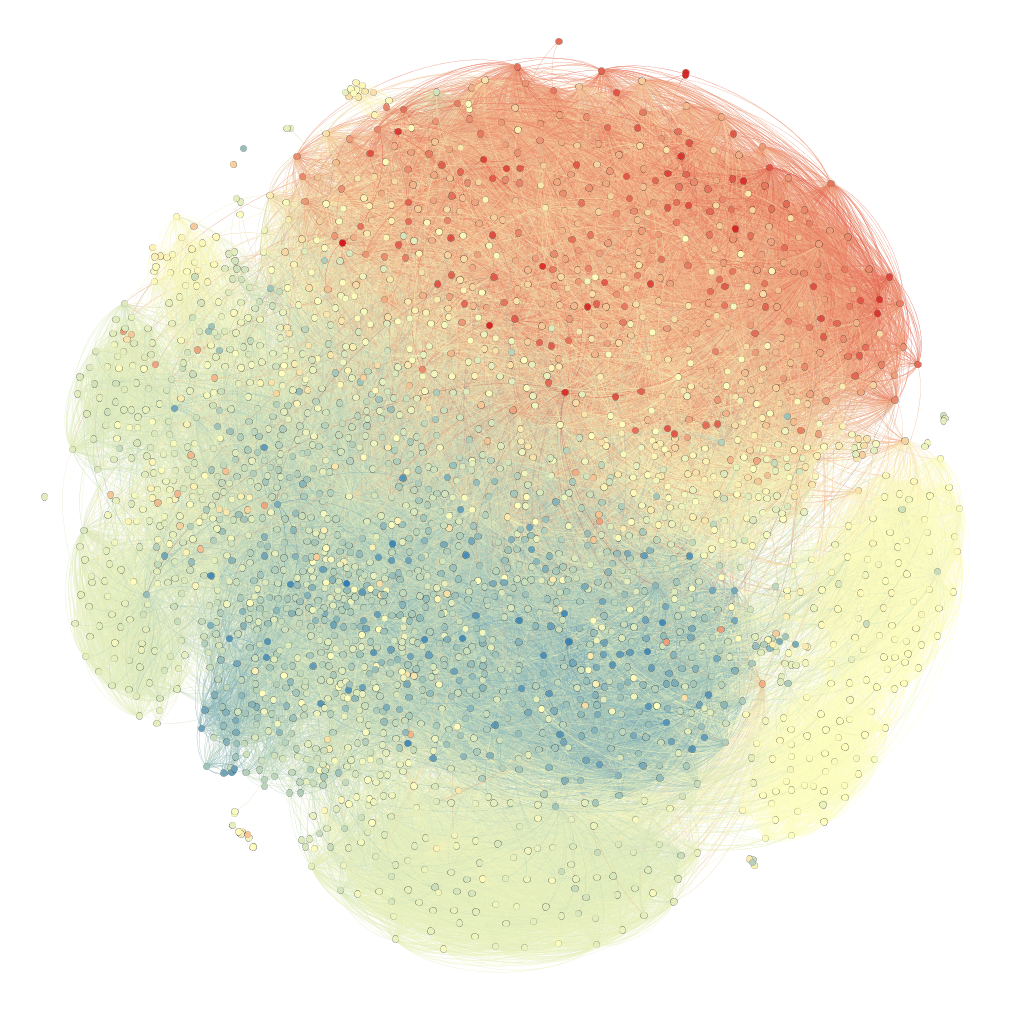
\includegraphics[width=1\linewidth]{figures/republican-democratic-graph.png}
  \caption{Partisanship Levels}
\label{fig:twitter-average-partisanship}
\end{subfigure}%
\begin{subfigure}{.24\textwidth}
  \centering
  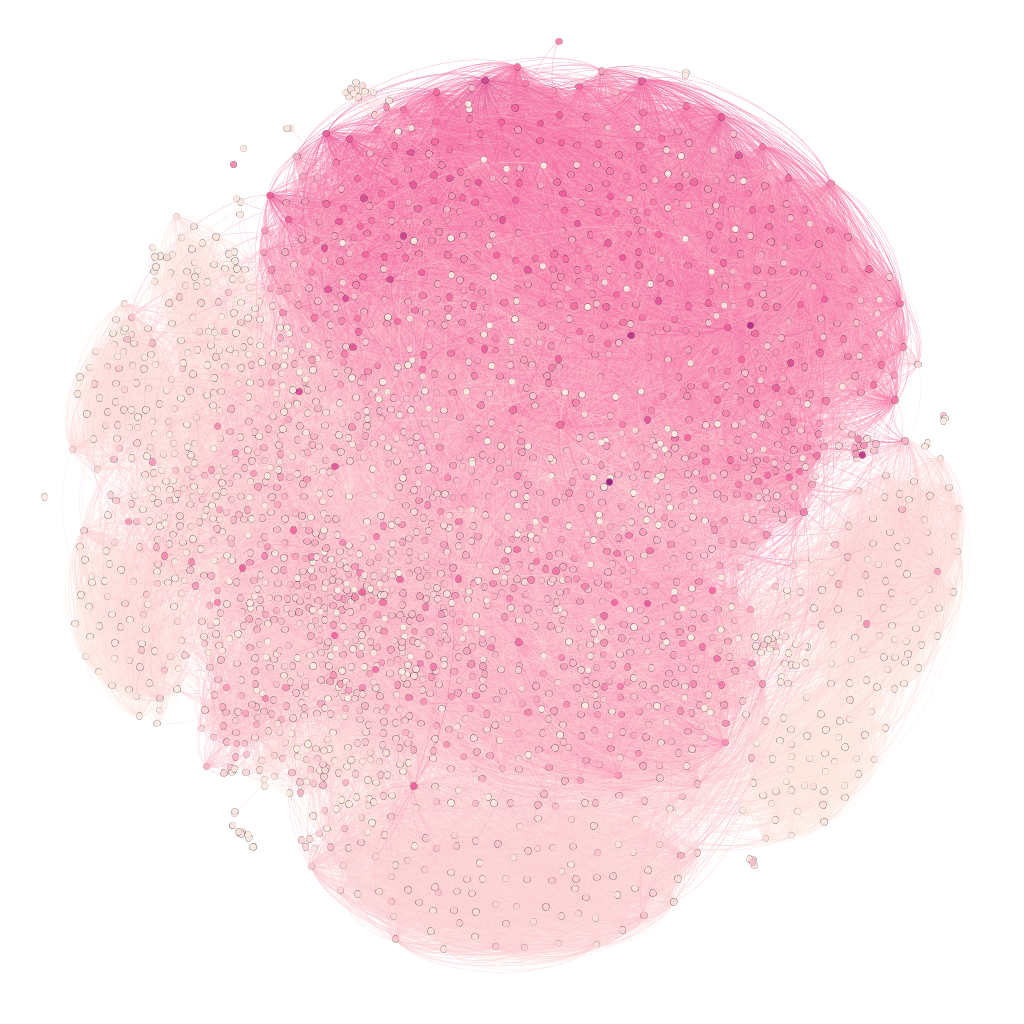
\includegraphics[width=1\linewidth]{figures/partisan-variance-graph.png}
  \caption{Partisanship Variance}
  \label{fig:twitter-variance-partisanship}
\end{subfigure}
\begin{subfigure}{.24\textwidth}
  \centering
  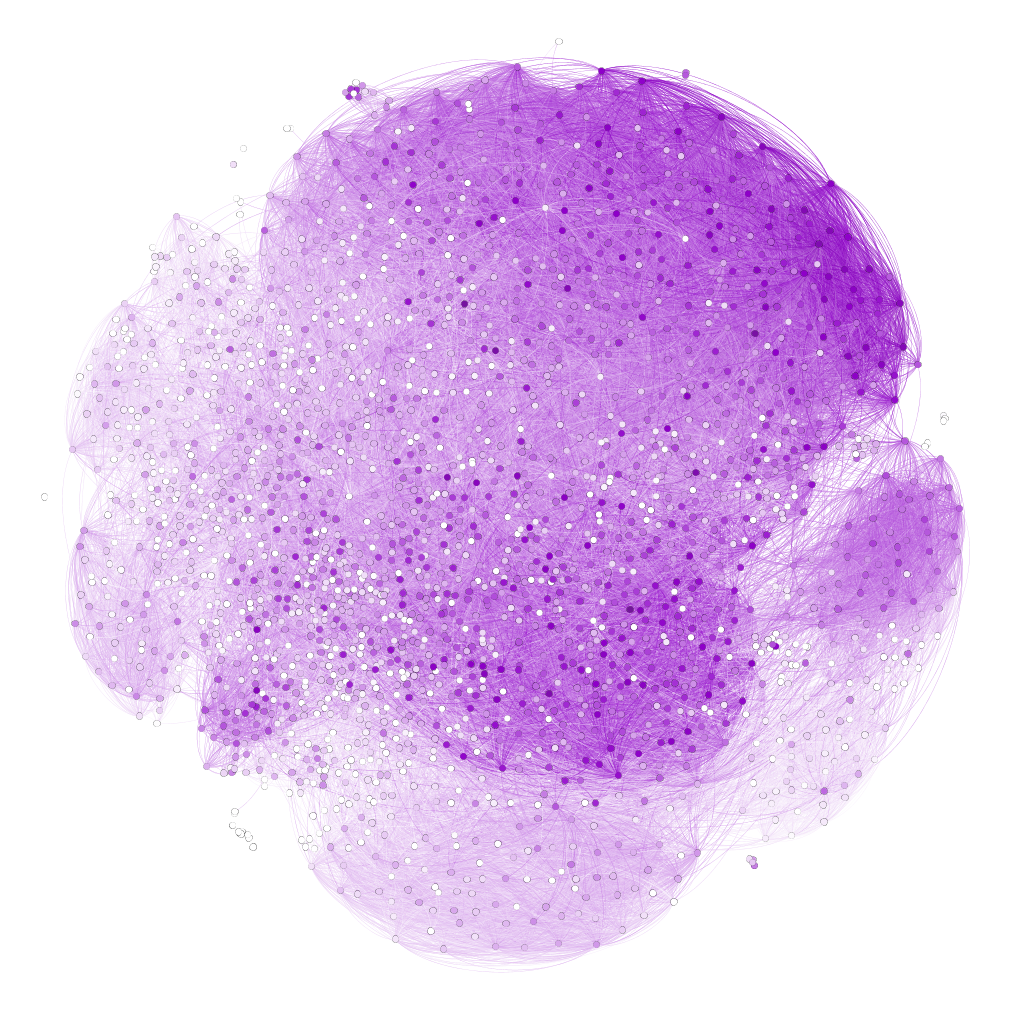
\includegraphics[width=1\linewidth]{figures/toxicity-graph.png}
  \caption{Perspective Toxicity }
  \label{fig:twitter-toxicity}
\end{subfigure}
\begin{subfigure}{.24\textwidth}
  \centering
  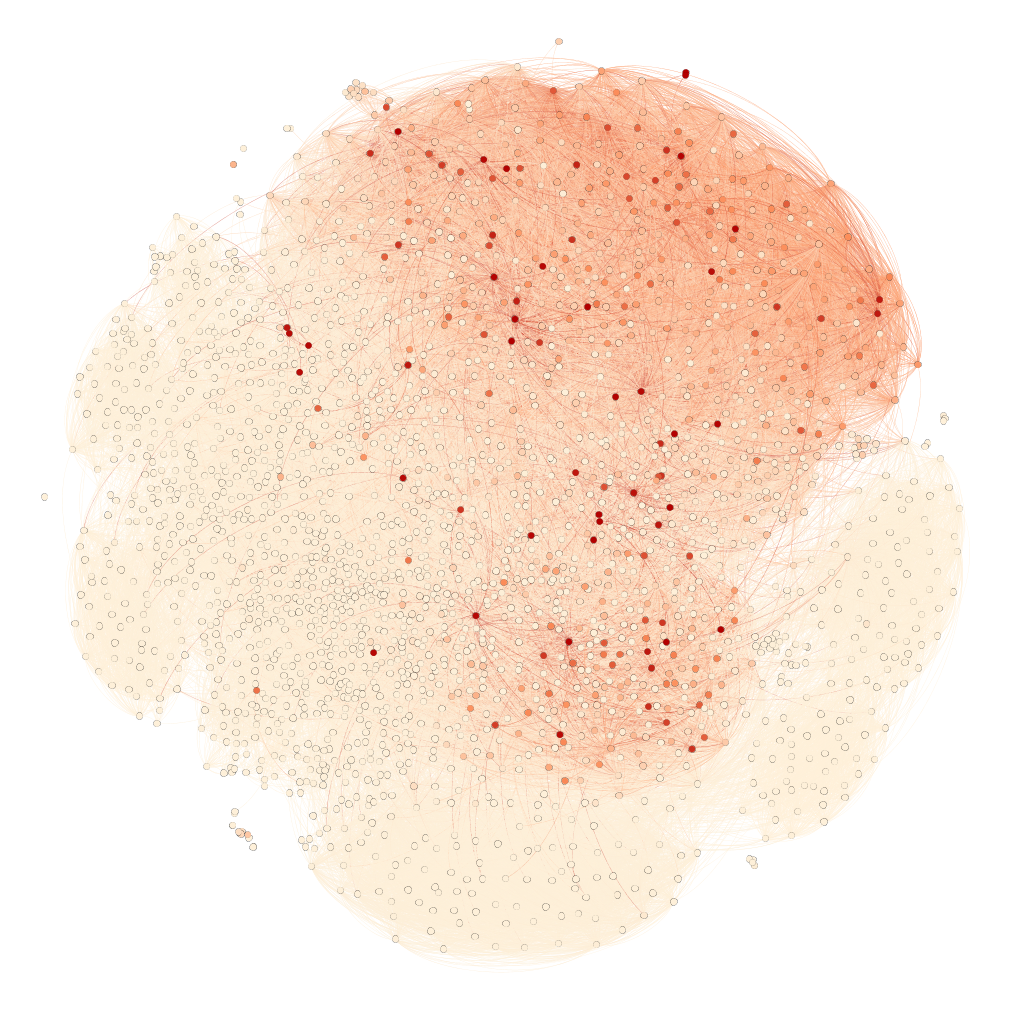
\includegraphics[width=1\linewidth]{figures/misinformation-graph.png}
  \caption{Misinformation }
  \label{fig:twitter-misinformation}
\end{subfigure}
\vspace{5pt}
\caption{\textbf{Interconnections between Twitter users with corresponding levels of partisanship, levels of sharing differently partisan sourced articles, toxicity, and levels of misinformation }-- As seen in the above graphs, highly conservative/Republican users and highly democratic/Republican users largely reference each other. Among these highly polarized communities, these users share more disparate and polarized articles, spread more misinformation, and are more toxic.
}
\label{fig:graph-correlations}
\end{figure*}

The tendency of user with higher levels of toxicity, higher levels of partisanship, and higher likelihoods to post misinformation further carries over to Twitter communities that many of these users participate in. Looking at the set of Twitter users in our scrape that posted at leas 300 URL (top 30K users in our dataset), we see this distinction visually. We plot Twitter mention graphs with edge weights based on how often each user mentions other users in their Tweets. Based on how often each user mentions another and clustering the graph using the Force Atlas 2 algorithm, we see two distinctive clusters of conservative/Republican and liberal/Democratic users form. As seen in Figure~\ref{fig:twitter-average-partisanship}, highly partisan users largely group and interact together, with conservative users mentioning other conservative users more frequently and vice versa. Looking a homophily (the tendency of users to mention/reference users of similar political bias as themselves) we see a moderately high value of 0.604. Comparing the graphs, in


As seen in Figure~\ref{fig:graph-correlations}, the cluster of highly liberal/Democratic and highly conservative/Republican users (Figure ~\ref{fig:twitter-average-partisanship}) corresponds to the set of users with higher amounts of political variance in the URLs that they tweet (Figure ~\ref{fig:twitter-variance-partisanship}) as well as the higher amounts of misinformation (Figure ~\ref{fig:twitter-misinformation}).

Looking at the graph of partisanship variance and the the graph of partisanship levels in Figure~\ref{fig:graph-correlations}, and the corresponding levels of correlation in between partisanship and partisanship variance, the most highly partisan accounts are the ones that hyperlink to a variety of different sources. This is particular true of Republican/conservative users. This can be most clearly seen in the dark pink cluster of the partisanship variance graph corresponding heavily with the Conservative/Republican red of the partisanship levels cluster, and finally dark orange cluster of the misinformation graph. 
